\documentclass[journal]{IEEEtran}
\usepackage[T1]{fontenc}
\usepackage[utf8]{inputenc}
\usepackage{booktabs,tabularx,array,multirow}
\usepackage{amsmath}
\usepackage{graphicx}
\usepackage{url}
\makeatletter\g@addto@macro\UrlBreaks{\do\_\do\-}\makeatother
\usepackage[hidelinks]{hyperref}
\newcolumntype{L}{>{\raggedright\arraybackslash}X}
\newcommand{\m}{$-$}

\begin{document}
\title{Supplementary Material for ``What Do Wrist-Worn Stress Detectors Detect? An Untrained Arousal Index Nearly Matches Them Across Five Empatica E4 Datasets''}
\author{Alvaro~Octavio~Ibarra~Reyes and Chen~Pan}
\maketitle
\renewcommand{\thesection}{S-\Roman{section}}
\renewcommand{\thetable}{S\Roman{table}}
\renewcommand{\thefigure}{S\arabic{figure}}
Section, table and figure numbers refer to this supplement. All values come from committed tables in \url{https://github.com/ALVAROI12/smartwatch-stress-detection}.

\section{Error budget and the chest-ECG bound}
\begin{table}[!t]
\centering
\caption{Test-Side Error Budget: Balanced-Accuracy Gain of Each Filter, Shapley-Averaged Over 24 Orders (HR/HRV/EDA)}
\label{tab:budget}
\footnotesize
\begin{tabularx}{\columnwidth}{@{}Lcccccc@{}}
\toprule
Dataset, model & All & F1 & F2 & F3 & F4 & Resid. \\
\midrule
PhysioNet, within & 0.776 & 0.003 & 0.007 & 0.020 & 0.020 & 0.175 \\
PhysioNet, external & 0.746 & 0.015 & 0.006 & 0.036 & 0.008 & 0.190 \\
Stress-Predict, within & 0.710 & 0.019 & 0.011 & 0.018 & 0.012 & 0.229 \\
Stress-Predict, external & 0.653 & 0.015 & \m0.015 & 0.012 & 0.005 & 0.329 \\
WESAD, external & 0.887 & 0 & 0.045 & 0 & 0.002 & 0.066 \\
\bottomrule
\end{tabularx}
\end{table}

\begin{figure}[!t]
\centering
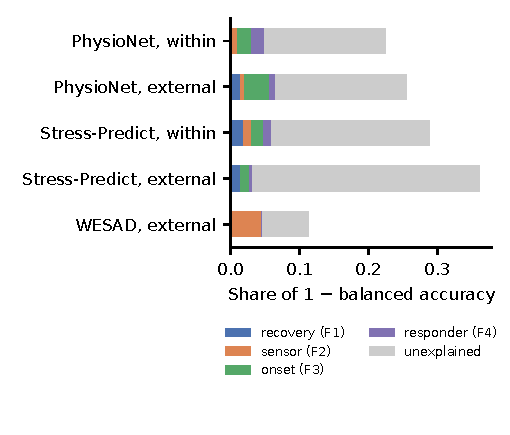
\includegraphics[width=\columnwidth]{fig_budget.pdf}
\caption{Error budget. Each bar is $1-$BA of the out-of-sample predictions; coloured segments are the Shapley-averaged gains of the four test-side filters, grey is the residual after all four. Negative gains (Stress-Predict external, F2) are drawn as zero.}
\label{fig:budget}
\end{figure}

Table~\ref{tab:budget} and Fig.~\ref{fig:budget} test four explanations for the low ceilings on PhysioNet and Stress-Predict as test-side filters on LOSO and external predictions: F1 drops rest windows within 5 min of a stressor offset (recovery contamination); F2 keeps windows with cardiac coverage of at least 0.5 (sensor loss); F3 drops the first 60 s of each stressor (onset latency); F4 keeps only subjects whose own stressor-minus-baseline heart rate or tonic EDA exceeds 0.5 baseline SD (non-response; label-using, diagnostic only). Together they buy 0.05--0.06 BA on PhysioNet and Stress-Predict (0.02 for the external model on Stress-Predict). With subject-bootstrap CIs (1000 draws; \texttt{rev8\_budget\_bootstrap\_ci.csv}), F1 and F3 exclude zero on Stress-Predict, F3 on external PhysioNet and F2 on WESAD; no single filter's upper bound exceeds 0.065 on PhysioNet or Stress-Predict. Without the label-using F4, the three label-free filters buy at most 0.056 (upper bound 0.09), and F4 adds at most 0.022 on top. The residual error of 0.17--0.23 (0.33 external on Stress-Predict; lower CI bounds 0.11--0.28) is explained by none of them. The responder filter is the one term sensitive to its definition (\texttt{partB\_responder\_sensitivity.csv}). At 0.5 or 1.0 baseline SD on either channel the two rules select the same subjects (32 of 35 PhysioNet, 32 of 34 Stress-Predict) and F4 gains 0.01--0.02. Requiring 1.0 SD on both channels keeps 17 of 35 PhysioNet subjects and raises within-dataset BA by 0.094 [0.05, 0.15] (external 0.065 [0.01, 0.13]); keeping the top half of subjects by pooled response gives 0.062 [0.01, 0.13]. On Stress-Predict the strict rules keep 12--17 of 34 subjects and gain 0.03 within (CI includes zero) and \m0.02 to +0.03 externally. Under the strict rules non-response is the largest single term on PhysioNet, about half of the four-filter total, yet the residual stays at 0.10--0.14 on PhysioNet and 0.21--0.35 on Stress-Predict. Onset latency and recovery are real but small: within-dataset Stress-Predict recall is 0.47 in the first minute of a stressor against 0.77 after 3 min, PhysioNet 0.63 in the first minute against 0.77 in the third, and rest false alarms peak in the first minute after offset (PhysioNet within 0.26 against 0.06--0.09 later); too few windows sit there to move BA.

On WESAD the only sizeable term is the sensor (F2, +0.045 external). Replacing wrist cardiac features with chest-ECG features on the same windows raises BA from 0.916 to 0.956 (AUROC 0.977 to 0.993), and chest ECG alone reaches 0.918, equal to the whole wrist pipeline; the gain concentrates in low-coverage windows, where wrist heart rate is absent (0.886 to 0.962). EDA alone gives 0.891. Motion-robust wrist heart rate is therefore worth at most about +0.04 on WESAD, and about 0.04 of error remains with chest-grade cardiac data.

\section{Leakage-controlled negative results}
\begin{table}[!t]
\centering
\caption{Leakage-Controlled Negative Results (Balanced Accuracy, HR/HRV/EDA Unless Stated)}
\label{tab:neg}
\footnotesize
\begin{tabularx}{\columnwidth}{@{}LL@{}}
\toprule
Question & Result \\
\midrule
Unsupervised domain adaptation (correlation alignment, maximum mean discrepancy, domain-adversarial and subject-adversarial networks), WESAD$\leftrightarrow$PhysioNet, physiology & 0.52--0.70 vs source-only 0.54--0.70; none reliably better \\
Few-shot on unseen dataset, first-in-time windows, $k=1$--5 per class & \m0.04 to +0.04 refit gain; none significant after Holm \\
Few-shot, random windows & only significant gains (WESAD $k=5$, +0.03); not deployable \\
Per-user threshold from calibration windows & hurts PhysioNet (\m0.08, $p_{\mathrm{holm}}<0.05$ at $k=3$) \\
Self-rated stress rise vs window recall (PhysioNet 54 units, WESAD 15) & PhysioNet $\rho$ = \m0.08 [\m0.42, 0.21] within, 0.02 [\m0.30, 0.31] external; WESAD \m0.49 [\m0.87, 0.17] within, \m0.60 [\m0.84, \m0.08] external (15 units); mild tasks not missed more \\
Detectability as a subject trait: recall across stressors & Stress-Predict $\rho$ = \m0.14 [\m0.51, 0.24]; PhysioNet 0.44 [\m0.04, 0.78] \\
Recall vs baseline HR, RMSSD, EDA, PPG coverage & $|\rho|\le 0.35$ with CIs including 0, except Stress-Predict external recall vs baseline EDA ($\rho=0.48$ [0.18, 0.70]) \\
Worst 20\% of subjects' share of misses & 37--61\% \\
Exercise absent from training (LODO with exercise as negatives) & 69.5\% of exercise windows called stress by the other-4 model; 4--6\% when PhysioNet's own subjects are in training (8--10\% under the panel's added-negative configuration, main-text Table III) \\
\bottomrule
\end{tabularx}
\end{table}

Table~\ref{tab:neg} collects results that close directions the literature has proposed. Unsupervised domain adaptation on top of per-subject normalisation does not beat source-only training in either direction between WESAD and PhysioNet, consistent with Kwon et al.~\cite{kwon2026}. Few-shot personalisation of a model trained on the other four datasets, with each user's first $k$ windows per class as calibration and a 30-s gap before any test window, adds at most 0.02--0.04 BA and nothing significant; drawing calibration windows at random from the recording produces the only significant gains, in line with Tervonen et al.~\cite{tervonen2026} and Akkaya~\cite{akkaya2026}. A per-user threshold hurts. Self-rated stress intensity does not predict which windows are missed: in PhysioNet, Stroop (mean rise 0.7 of 10) is detected as well as arithmetic (2.5); WESAD's negative correlation rests on the two subjects with the largest rise. The data give no support to detectability as a stable subject trait: recall is not correlated across stressors, is not predicted by baseline physiology or PPG coverage (one exception, Stress-Predict external recall against baseline EDA), and misses are only moderately concentrated; PhysioNet's within and external models do agree on who is hard ($\rho=0.64$ [0.37, 0.82]).


\begin{thebibliography}{9}
\bibitem{akkaya2026} A. Akkaya, ``Calibration, not architecture, limits cross-subject wearable stress detection: A multi-dataset, decision-focused evaluation with label-efficient recalibration,'' \emph{BMC Med. Inform. Decis. Mak.}, 2026, doi: 10.1186/s12911-026-03842-1 (abstract only).
\bibitem{kwon2026} N. Kwon, S. Yoon, J. Hur, and H. S. Kang, ``When wellness stress detection enters healthcare workflows: An iso-heart-rate, cross-corpus evaluation of wrist wearables,'' \emph{Healthcare}, vol. 14, no. 15, Art. no. 2434, 2026, doi: 10.3390/healthcare14152434.
\bibitem{tervonen2026} J. Tervonen, E. Amparore, M. Botta, J. N\"arv\"ainen, K. Pettersson, and J. M\"antyj\"arvi, ``Data-constrained personalization of cognitive state detection with feature-based and foundation models,'' \emph{User Model. User-Adapt. Interact.}, 2026, doi: 10.1007/s11257-026-09444-w.
\end{thebibliography}
\end{document}
